\subsection{Adição de arcos}

\begin{proposition}
\label{prop:seno-e-cosseno-da-soma}
    Sejam $\alpha, \beta \in \R$. Então
$$\cos \paren{\alpha + \beta} = \cos \alpha \cdot \cos \beta - \sen
\alpha \cdot \sen \beta$$ e
$$\sen \paren{\alpha + \beta} = \sen \alpha \cdot \cos \beta +\sen \beta \cdot
\cos \alpha.$$
\end{proposition}

\begin{proof}
    Sejam $\alpha, \beta \in \reais$. Consideremos, incialmente, o caso em que 
    $\alpha,\beta>0$ e $\alpha+\beta < \frac{\pi}{2}$. Ele é ilustrado na Imagem~\ref{img:prova-seno-e-cosseno-da-soma}.
    %
    \begin{figure}[H]
        \centering
        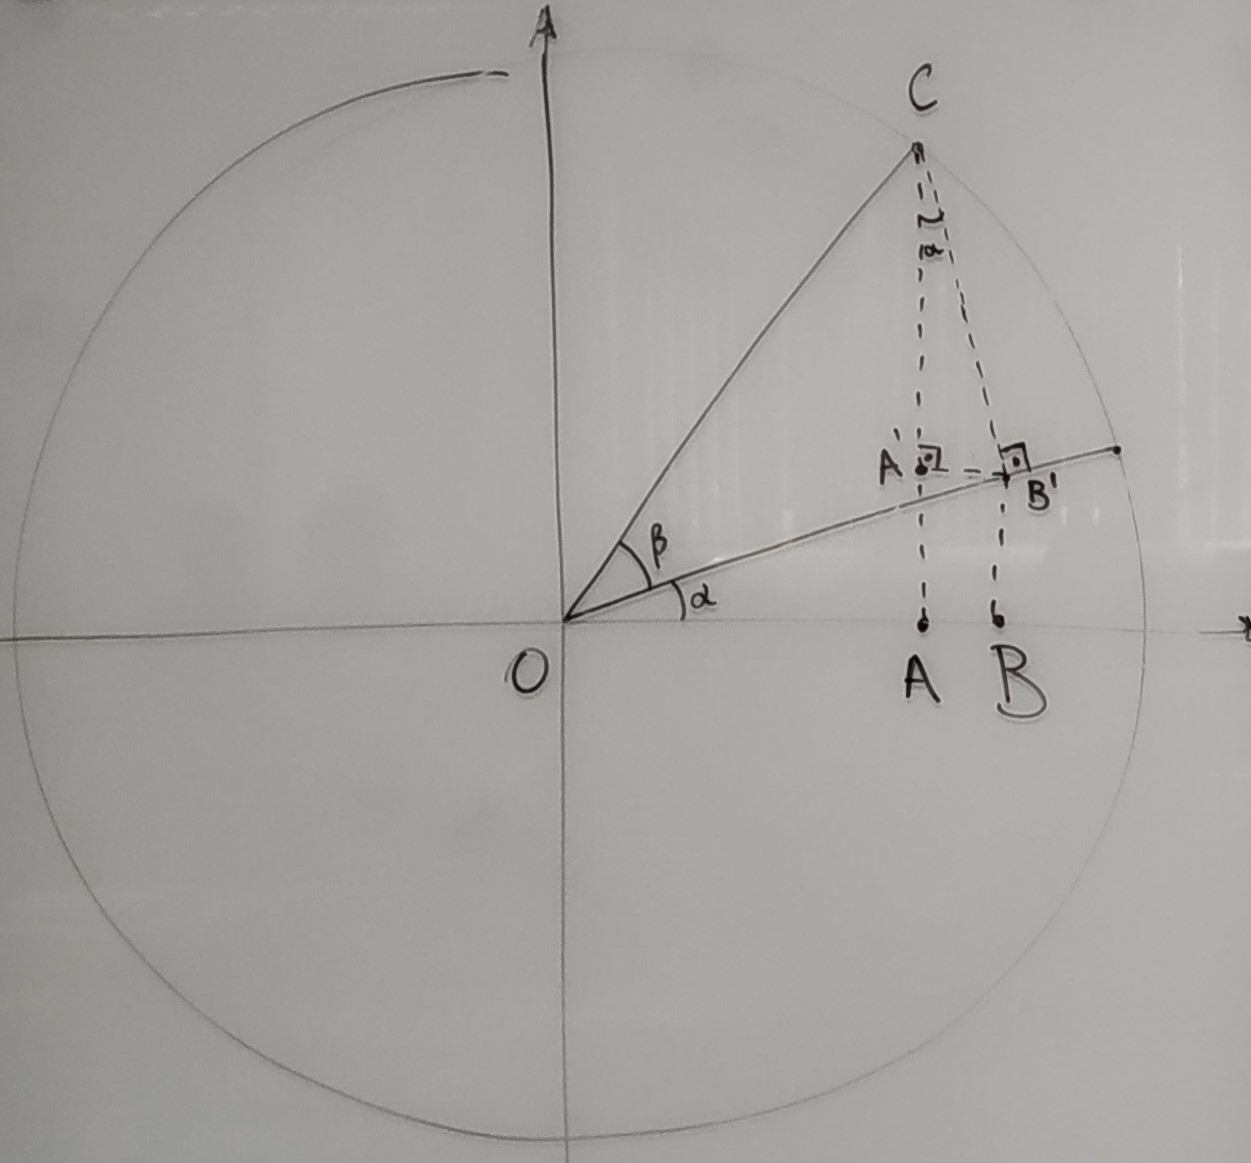
\includegraphics[scale=0.20]{\imgdirfromsection/fig-c10-prop14-recortada.jpg}
        \caption{Ângulos $\alpha$ e $\beta$ e pontos $O$, $A$, $A^\prime$, $B$, $B^\prime$ e $C$.}
        \label{img:prova-seno-e-cosseno-da-soma}
    \end{figure}
    %
    Da imagem, obtemos as seguintes igualdades:
    %
    \begin{equation*}
        \cos(\alpha+\beta) = \seg{OA}
    \end{equation*}
    %
    \begin{equation}
    \label{eq:prova-prop-seno-cosseno-soma-2}
        \cos\beta = \seg{OB^{\prime}}
    \end{equation}
    %
    \begin{equation}
    \label{eq:prova-prop-seno-cosseno-soma-3}
        \sen\beta = \seg{CB^{\prime}}
    \end{equation} 
    %
    \begin{equation}
    \label{eq:prova-prop-seno-cosseno-soma-4}
        \sen\alpha = \frac{\seg{A^{\prime}B^{\prime}}}{\seg{CB^{\prime}}}
    \end{equation}
    %
    \begin{equation}
    \label{eq:prova-prop-seno-cosseno-soma-5}
        \cos\alpha = \frac{\seg{OB}}{\seg{OB^{\prime}}}
    \end{equation}

    De \ref{eq:prova-prop-seno-cosseno-soma-3} e \ref{eq:prova-prop-seno-cosseno-soma-4}, temos que:
    %
    \begin{equation}
    \label{eq:prova-prop-seno-cosseno-soma-6}
        \seg{A^{\prime} B^{\prime}} = \sen \alpha \sen \beta
    \end{equation}

    De \ref{eq:prova-prop-seno-cosseno-soma-2} e \ref{eq:prova-prop-seno-cosseno-soma-5}, temos que:
    %
    \begin{equation}
    \label{eq:prova-prop-seno-cosseno-soma-7}
        \seg{OB} = \cos \alpha \cos \beta
    \end{equation}

    Pela imagem, temos, além disso, que:
    %
    \begin{equation}
    \label{eq:prova-prop-seno-cosseno-soma-8}
        \seg{OA} = \seg{OB} - \seg{AB}
    \end{equation}


    Note, agora, que:
    %
    \begin{align*}
        \cos(\alpha + \beta) &= \frac{\seg{OA}}{\seg{OC}} \\
        &= \seg{OA} \\
        &\stackrel{\ref{eq:prova-prop-seno-cosseno-soma-8}}{=} \seg{OB} - \seg{AB} \\
        &\stackrel{\ref{eq:prova-prop-seno-cosseno-soma-7}}{=}  \cos \alpha \cos \beta - \seg{AB} \\
        &= \cos \alpha \cos \beta - \seg{A^{\prime}B^{\prime}} \\
        &\stackrel{\ref{eq:prova-prop-seno-cosseno-soma-6}}{=}  \cos \alpha \cos \beta - \sen \alpha \sen \beta
    \end{align*}

    Considere as relações:
    %
    \begin{equation}
    \label{eq:prova-prop-seno-cosseno-soma-9}
        \cos\prn{t+\frac \pi 2} = -\sen t
    \end{equation}
    %
    \begin{equation}
    \label{eq:prova-prop-seno-cosseno-soma-10}
        \sen\prn{t+\frac \pi 2} = \cos t
    \end{equation}

    Temos que:
    %
    \begin{align*}
        \sen(\alpha + \beta ) & \stackrel{\ref{eq:prova-prop-seno-cosseno-soma-9}}{=} -\cos\prn{\alpha + \beta + \frac \pi 2} \\
        & = -\bracket{\cos \alpha\cdot \cos\prn{\beta + \frac \pi 2} - \sin \alpha \cdot \sin\prn{\beta + \frac \pi 2}}\\
        &\stackrel{\ref{eq:prova-prop-seno-cosseno-soma-9}}{=} -\bracket{\cos \alpha\cdot \prn{-\sen \beta} - \sin \alpha \cdot \sin\prn{\beta + \frac \pi 2}}\\
        &\stackrel{\ref{eq:prova-prop-seno-cosseno-soma-10}}{=} \cos \alpha \sen \beta + \sen \alpha \cos \beta
    \end{align*}
    


\end{proof}

\begin{remark}
    Da Proposição~\ref{prop:seno-e-cosseno-da-soma} e da (im)paridade das funções seno e cosseno 
    (Definição~\ref{def:funcao-par-impar}) seguem, para todos $\alpha, \beta \in \reais$, que:

$$\cos \paren{\alpha - \beta} = \cos \alpha \cdot \cos \beta + \sen
\alpha \cdot \sen \beta$$ e
$$\sen \paren{\alpha - \beta} = \sen \alpha \cdot \cos \beta - \sen \beta \cdot
\cos \alpha.$$

Além disso, temos os casos particulares:
$$\cos \paren{2\alpha } = \cos^2 \alpha  - \sen^2 \alpha \ \ \text{ e }
\ \ \sen \paren{2\alpha } = 2\sen \alpha \cdot \cos \alpha.$$
\end{remark}

\import{}{rotacao-de-pontos}